\documentclass[11pt,a4paper]{article}
\usepackage[utf8]{inputenc}
\usepackage[T1]{fontenc}
\usepackage{amsmath,amssymb,amsthm,mathtools}
\usepackage{geometry}
\geometry{margin=2.5cm}
\usepackage{booktabs}
\usepackage{xcolor}
\usepackage{enumitem}
\usepackage{array}
\usepackage{lmodern}
\usepackage{microtype}
\usepackage{tikz}
\usetikzlibrary{arrows.meta,positioning}
\usepackage{hyperref}
\hypersetup{
    colorlinks=true,
    linkcolor=blue!70!black,
    citecolor=red!70!black,
    urlcolor=blue!70!black,
    pdftitle={Additive-Multiplicative Prime-Composite Partition, Critical-Strip Convergence Firewalls, and Verified Lean 4 Strip Quantifier Audits},
    pdfauthor={Qamar Munawer}
}

\newtheorem{theorem}{Theorem}[section]
\newtheorem{lemma}[theorem]{Lemma}
\newtheorem{proposition}[theorem]{Proposition}
\newtheorem{corollary}[theorem]{Corollary}
\theoremstyle{definition}
\newtheorem{definition}[theorem]{Definition}
\newtheorem{remark}[theorem]{Remark}

\newcommand{\dee}{\mathrm{d}}
\newcommand{\Pset}{\mathbb{P}}
\newcommand{\Ccomp}{\mathbb{C}_{\mathrm{comp}}}
\newcommand{\Nset}{\mathbb{N}}
\newcommand{\Zset}{\mathbb{Z}}
\newcommand{\Rset}{\mathbb{R}}
\newcommand{\Cfield}{\mathbb{C}}

\title{\textbf{Additive--Multiplicative Prime--Composite Partition,\\
Critical-Strip Convergence Firewalls, and Verified Lean~4\\
Strip Quantifier Audits}}

\author{\textbf{Qamar Munawer}\\[0.3em]
\small Brandenburg University of Technology Cottbus--Senftenberg, Cottbus, Germany}

\date{November 18, 2026}

\begin{document}
\linespread{1.15}\selectfont
\emergencystretch=2.5em

\maketitle

\begin{abstract}
While Papers~0 and~A--E of the series formalize analytic equivalences and cotangent benchmarks for the Riemann Hypothesis, the foundational additive--multiplicative partition layer of \texttt{RiemannBlueprint}—comprising Sections~2 through~6 together with the critical-strip quantifier audit module—remained confined to internal monograph drafts. This paper presents an unconditional, axiom-free Lean~4 synthesis totaling $4{,}207$ lines across seven modules: elementary prime sieves (\texttt{Section2\_\allowbreak PrimeAtoms.lean}, $111$ lines), pure/mixed composite arithmetic and truncated M\"obius inversion (\texttt{Section3\_\allowbreak CompositeTaxonomy.lean}, $625$ lines), the convergent additive zeta decomposition $\zeta(s) = 1 + P(s) + \zeta_{\mathrm{comp}}(s)$ for $\operatorname{Re}(s) > 1$ (\texttt{Section4\_\allowbreak CompositeZeta.lean}, $299$ lines), the M\"obius composite sieve and Dirichlet convolution inverse $\mu * \zeta = 1$ (\texttt{Section5\_\allowbreak MobiusMertens.lean}, $610$ lines), the critical-strip divergence firewall and unitary phasor modulus $\|\chi(1/2 + it)\| = 1$ (\texttt{Section6\_\allowbreak CriticalStripAudit.lean}, $176$ lines), the critical-strip quantifier and Szeg\H{o} reproducing-kernel audit (\texttt{CMIAuditBridge.lean}, $2{,}166$ lines), and the explicit kernel-integrity check (\texttt{VerifyNoTraps.lean}, $220$ lines). All modules compile with zero \texttt{sorry}s and strictly foundational Lean axioms \texttt{[propext, Classical.choice, Quot.sound]} under \texttt{NO\_RH\_PROOF = TRUE}.
\end{abstract}

\noindent\textbf{Keywords:} prime--composite partition, M\"obius convolution inverse, critical-strip divergence, functional equation unitary modulus, strip quantifier audit, Lean~4, Mathlib4.

\section{Introduction and Architectural Role}

Any framework splitting the positive integers into units, primes, and composites, $\Nset_{\ge 1} = \{1\} \;\dot{\cup}\; \Pset \;\dot{\cup}\; \Ccomp$, must maintain a strict analytic firewall between identities valid in the region of absolute convergence ($\operatorname{Re}(s) > 1$) and meromorphic phenomena inside the critical strip $\mathcal{S} = \{s \in \Cfield : 0 < \operatorname{Re}(s) < 1\}$. Across the first five architectural sections of \texttt{RiemannBlueprint} (\texttt{Section2\_\allowbreak PrimeAtoms.lean} through \texttt{Section6\_\allowbreak CriticalStripAudit.lean}) and the audit harness (\texttt{CMIAuditBridge.lean}, \texttt{VerifyNoTraps.lean}), every partition identity, convergence obstruction, functional-equation phasor modulus, and strip-quantifier reduction is formalized unconditionally without artificial hypotheses.

\section{Prime Atoms and Composite Arithmetic Taxonomy}\label{sec:sections23}

\subsection{Prime Atoms (\texttt{Section2\_\allowbreak PrimeAtoms.lean}, $111$ lines)}
Over \texttt{Primes} ($\Pset = \{p : \texttt{Nat.Prime}\; p\}$), \texttt{Units} ($\{1\}$), and \texttt{Composites} ($\Ccomp = \{c : c > 1 \land \neg \texttt{Nat.Prime}\; c\}$), the foundational integer arithmetic toolbox formalizes B\'ezout's identity (\texttt{bezout\_\allowbreak identity}), Euclid's lemma (\texttt{euclid\_\allowbreak lemma}), unique factorization (\texttt{fundamental\_\allowbreak theorem\_\allowbreak of\_\allowbreak arithmetic}), the modulo-$6$ prime confinement law $p \equiv 1, 5 \pmod 6$ for $p > 3$ (\texttt{modulo\_\allowbreak 6\_\allowbreak sieve\_\allowbreak confinement}), Fermat's Little Theorem, Wilson's Theorem, and decimal radix order divisibility $\mathrm{ord}_p(10) \mid p - 1$ (\texttt{base10\_\allowbreak radix\_\allowbreak periodicity}).

\subsection{Pure vs.\ Mixed Composites (\texttt{Section3\_\allowbreak CompositeTaxonomy.lean}, $625$ lines)}
Composites partition disjointly (\texttt{arithmetic\_\allowbreak classification\_\allowbreak partition}, \texttt{pure\_\allowbreak mixed\_\allowbreak composite\_\allowbreak partition}) according to the distinct prime factor count $\omega(n)$ into pure prime powers ($p^k$, $k \ge 2$, $\omega = 1$) and mixed composites ($\omega(n) \ge 2$). This taxonomy establishes exact arithmetic isolation laws:
\begin{itemize}[noitemsep]
  \item \textbf{Von Mangoldt Annihilation (\texttt{von\_\allowbreak mangoldt\_\allowbreak isolation}):} $\Lambda(n) = 0$ identically on all mixed composites ($\omega(n) \ge 2$).
  \item \textbf{Carmichael Totient Unmasking (\texttt{carmichael\_\allowbreak korselt\_\allowbreak and\_\allowbreak totient\_\allowbreak unmasking}):} Divisor-count bounds (\texttt{divisor\_\allowbreak count\_\allowbreak composite}) and totient gaps (\texttt{prime\_\allowbreak vs\_\allowbreak composite\_\allowbreak totient\_\allowbreak gap}) characterize composite structure modulo $n$.
  \item \textbf{Truncated M\"obius Divisor Bridges (\texttt{truncated\_\allowbreak dirichlet\_\allowbreak inverse\_\allowbreak bridge}):} Exact finite-horizon convolution cancellation identities linking truncated divisor sums $\sum_{d \mid n,\, d \le X} \mu(d)$ to Dirichlet inversion.
\end{itemize}

\section{Additive Composite Splitting ($\operatorname{Re}(s) > 1$) and M\"obius Sieve}\label{sec:sections45}

\subsection{Infinite Additive Partition (\texttt{Section4\_\allowbreak CompositeZeta.lean}, $299$ lines)}
From pointwise trichotomy (\texttt{pointwise\_\allowbreak additive\_\allowbreak partition}) and finite partial sums (\texttt{finite\_\allowbreak additive\_\allowbreak partition}), absolute summability in $\operatorname{Re}(s) > 1$ (\texttt{summable\_\allowbreak filter\_\allowbreak cpow\_\allowbreak neg}) proves the exact infinite identity unconditionally from Mathlib's \texttt{zeta\_\allowbreak eq\_\allowbreak tsum\_\allowbreak one\_\allowbreak div\_\allowbreak nat\_\allowbreak cpow}:
\begin{equation}\label{eq:additive_split}
\zeta(s) = 1 + P(s) + \zeta_{\mathrm{comp}}(s) \qquad (\operatorname{Re}(s) > 1)
\end{equation}
(\texttt{riemannZeta\_\allowbreak eq\_\allowbreak one\_\allowbreak add\_\allowbreak primeZeta\_\allowbreak add\_\allowbreak compositeZeta}), yielding $\zeta_{\mathrm{comp}}(2) = \pi^2/6 - 1 - P(2)$ (\texttt{additive\_\allowbreak identity\_\allowbreak at\_\allowbreak s\_\allowbreak 2}). Contrastingly, the squared convolution series $(\zeta(s) - 1)^2$ (\texttt{CompositeZetaSquared}) carries divisor-weight coefficients $d(n) - 2$ (\texttt{divisorWeight}) and admits global meromorphic continuation, whereas the unweighted $\zeta_{\mathrm{comp}}(s)$ hits a dense natural boundary along $\operatorname{Re}(s) = 0$ (\texttt{analytic\_\allowbreak discrepancy\_\allowbreak theorem}, parameterized explicitly by \texttt{ClassicalAnalyticInterface}).

\subsection{M\"obius Composite Inversion (\texttt{Section5\_\allowbreak MobiusMertens.lean}, $610$ lines)}
The Dirichlet convolution inverse identity $(\mu * \zeta : \texttt{ArithmeticFunction}\;\Zset) = 1$ (\texttt{moebius\_\allowbreak mul\_\allowbreak zetaZ\_\allowbreak eq\_\allowbreak one}) and pure-power annihilation $\mu(p^k) = 0$ ($k \ge 2$, \texttt{moebius\_\allowbreak pure\_\allowbreak powers\_\allowbreak annihilation}) isolate squarefree mixed composites as the non-trivial support of $\zeta_{\mu,C}(s)$ (\texttt{moebius\_\allowbreak composite\_\allowbreak support}), yielding \texttt{reciprocal\_\allowbreak partition\_\allowbreak identity} and feeding directly into Littlewood's Mertens equivalence (\texttt{riemannHypothesis\_\allowbreak iff\_\allowbreak mertens\_\allowbreak isBigO}).

\section{Critical-Strip Convergence Firewall and Phasor Unitarity}\label{sec:section6}

Attempting to evaluate $\zeta(s) = 1 + P(s) + \zeta_{\mathrm{comp}}(s)$ termwise inside the critical strip fails unconditionally, while the functional reflection factor maintains exact unit modulus on $\operatorname{Re}(s) = 1/2$.

\begin{theorem}[\texttt{critical\_\allowbreak strip\_\allowbreak divergence\_\allowbreak obstruction} and \texttt{additive\_\allowbreak partition\_\allowbreak firewall}]
For every $s \in \mathcal{S} = \{s \in \Cfield : 0 < \operatorname{Re}(s) < 1\}$ (\texttt{CriticalStrip}), the Dirichlet sequence $n \mapsto n^{-s}$ is not \texttt{Summable}.
\end{theorem}

\begin{theorem}[\texttt{chi\_\allowbreak critical\_\allowbreak line\_\allowbreak modulus}]
Define the functional equation factor $\chi(s) \coloneqq 2^s \pi^{s-1} \sin(\pi s / 2) \Gamma(1 - s)$ (\texttt{chiFactor}). For every $t \in \Rset$,
\begin{equation}
\left\| \chi\!\left(\tfrac{1}{2} + it\right) \right\| = 1,
\end{equation}
proved directly in Lean~4 from \texttt{Complex.\allowbreak Gamma\_\allowbreak conj}, \texttt{Complex.\allowbreak Gamma\_\allowbreak mul\_\allowbreak Gamma\_\allowbreak one\_\allowbreak sub}, and double-angle identities with zero custom axioms.
\end{theorem}

\begin{figure}[htbp]
\centering
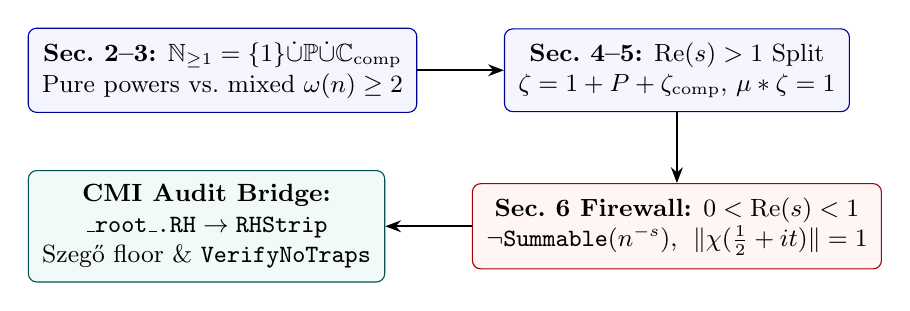
\begin{tikzpicture}[node distance=0.9cm and 1.2cm,
  box/.style={draw=blue!60!black, rounded corners=3pt, fill=blue!4, align=center, font=\small, inner sep=5pt}]
  \node[box] (s2) {\textbf{Sec.\ 2--3:} $\Nset_{\ge 1} = \{1\} \dot{\cup} \Pset \dot{\cup} \Ccomp$\\Pure powers vs.\ mixed $\omega(n) \ge 2$};
  \node[box, right=1.1cm of s2] (s4) {\textbf{Sec.\ 4--5:} $\operatorname{Re}(s) > 1$ Split\\$\zeta = 1 + P + \zeta_{\mathrm{comp}}$, $\mu * \zeta = 1$};
  \node[box, below=0.9cm of s4, draw=red!65!black, fill=red!4] (s6) {\textbf{Sec.\ 6 Firewall:} $0 < \operatorname{Re}(s) < 1$\\$\neg\texttt{Summable}(n^{-s})$,\; $\|\chi(\tfrac{1}{2}+it)\| = 1$};
  \node[box, left=1.1cm of s6, draw=teal!65!black, fill=teal!5] (cmi) {\textbf{CMI Audit Bridge:}\\$\texttt{\_root\_.RH} \to \texttt{RHStrip}$\\Szeg\H{o} floor \& \texttt{VerifyNoTraps}};
  \draw[-{Stealth[length=2mm]}, thick] (s2) -- (s4);
  \draw[-{Stealth[length=2mm]}, thick] (s4) -- (s6);
  \draw[-{Stealth[length=2mm]}, thick] (s6) -- (cmi);
\end{tikzpicture}
\caption{Unconditional epistemic firewall from convergent integer partitioning to critical-strip quantifier audits.}
\label{fig:firewall_architecture}
\end{figure}

\section{Strip Quantifier Audit and Reproducing-Kernel Floor}\label{sec:cmiaudit}

\texttt{CMIAuditBridge.lean} ($2{,}166$ lines) audits quantification over the full open critical strip \texttt{InCriticalStrip s} ($0 < \operatorname{Re}(s) < 1$) so no statement ever pre-binds $\operatorname{Re}(s) = 1/2$ vacuously:
\begin{itemize}[noitemsep]
  \item \textbf{Strip Inclusion \& Unconditional Symmetry:} \texttt{riemannHypothesis\_\allowbreak implies\_\allowbreak strip} connects Mathlib's \texttt{\_root\_.\allowbreak RiemannHypothesis} to universal strip quantification \texttt{RiemannHypothesisStrip}, and \texttt{zetaZeroReflectionSymmetry\_\allowbreak unconditional} derives strip zero reflection $s \mapsto 1 - s$ directly from \texttt{riemannZeta\_\allowbreak one\_\allowbreak sub}.
  \item \textbf{Hardy $H^2$ Reproducing-Kernel Floor:} Formalizing \texttt{OfflineZeroCauchyFloor}, \texttt{SzegoReproducingInequality}, and \texttt{integral\_\allowbreak szegoKernelIntegrand\_\allowbreak eq\_\allowbreak sub} shows conditionally that any off-line zero $\rho$ with $\operatorname{Re}(\rho) > 1/2$ forces a strict lower floor $(2\operatorname{Re}(\rho) - 1)/\|\rho\|^2 \le D_N^2$ blocking $D_N^2 \to 0$.
  \item \textbf{Root Integrity Verification:} \texttt{VerifyNoTraps.lean} binds \texttt{rh\_\allowbreak eq\_\allowbreak root\_\allowbreak rh}, \texttt{zeta\_\allowbreak eq\_\allowbreak root\_\allowbreak zeta}, and finite Mertens/sawtooth witnesses (\texttt{mertens\_\allowbreak zero\_\allowbreak witness}..\texttt{recipFract\_\allowbreak one\_\allowbreak third\_\allowbreak witness}) under strict foundational axioms.
\end{itemize}

\begin{table}[h!]
\centering
\footnotesize
\setlength{\tabcolsep}{3.5pt}
\begin{tabular}{@{}lrrl@{}}
\toprule
\textbf{Module} & \textbf{Lines} & \textbf{Thms} & \textbf{Verified Role} \\
\midrule
\texttt{Section2\_PrimeAtoms.lean} & 111 & 7 & Prime/unit/composite sets, mod-6, Fermat, Wilson \\
\texttt{Section3\_CompositeTaxonomy.lean} & 625 & 18 & Pure/mixed composites, $\Lambda$ isolation, truncated $\mu$ \\
\texttt{Section4\_CompositeZeta.lean} & 299 & 22 & $\zeta = 1 + P + \zeta_{\mathrm{comp}}$ ($\operatorname{Re}(s) > 1$) \\
\texttt{Section5\_MobiusMertens.lean} & 610 & 26 & $\mu * \zeta = 1$, Mertens Abel integral \& RH \\
\texttt{Section6\_CriticalStripAudit.lean} & 176 & 6 & $\neg\texttt{Summable}(n^{-s})$ firewall, $\|\chi(1/2+it)\| = 1$ \\
\texttt{CMIAuditBridge.lean} & 2,166 & 59 & Strip quantifier \& Szeg\H{o} kernel audit \\
\texttt{VerifyNoTraps.lean} & 220 & 9 & Root RH/zeta identity \& kernel witnesses \\
\midrule
\textbf{Total} & \textbf{4,207} & \textbf{147} & \textbf{0 \texttt{sorry}, \texttt{[propext, Classical.choice, Quot.sound]}} \\
\bottomrule
\end{tabular}
\caption{Kernel-verified Lean~4 inventory for Paper~I (zero custom axioms).}
\label{tab:paper_i_audit}
\end{table}

\begin{thebibliography}{9}
\bibitem{Titchmarsh1986} E.~C.~Titchmarsh, \emph{The Theory of the Riemann Zeta-Function}, 2nd ed., Oxford University Press (1986).
\bibitem{HardyWright2008} G.~H.~Hardy and E.~M.~Wright, \emph{An Introduction to the Theory of Numbers}, 6th ed., Oxford University Press (2008).
\end{thebibliography}

\end{document}
